\let\textcircled=\pgftextcircled
\chapter{Metastable state selection for Hidden Markov Models}
\label{chap:hmm}


\begin{table}
    \centering
    \mycaption[Important symbols]{\textsc{Important symbols used throughout this chapter}.}
    \begin{tabularx}{0.9\textwidth}{ |l| >{\raggedright\arraybackslash}X | } 
    \hline
    \textbf{Symbol}  &  \textbf{Definition} \\
    \hline\hline
    $g$ & Number of hidden states in a HMM. \\
    $n$ & Number of observed states in a HMM. \\
    $\mathbf{\tilde{T}}$ & The $g\times g$ HMM transition matrix. \\
    $\mathbf{E}$ & The $g \times n$ emission matrix. $E_{ij}$ is the probability of observing a state $j$ given an hidden state $i$. \\
    $\tilde{\bm{\pi}}$ & Stationary distribution of hidden states \\
    $\{s_{t}\}$ & Trajectory of observed states \\
    $\{h_{t}\}$ & Trajectory of hidden states \\
    $p(\{s_t\}|M)$ & The integrated or marginal observed likelihood: the probability of observing $\{s_t\}$ given the model $M$. \\
    $p(\{(s_t, h_t)\}|M)$ & The integrated or marginal complete-data likelihood: the probability of observing both $\{s_t\}$ and $\{h_t\}$ given the model $M$.  \\
    $L(\tilde{\mathbf{T}}, \mathbf{E}| \{s_t\})$ & The HMM likelihood. \\
    $\theta$ & The HMM parameters, $\tilde{\mathbf{T}}$ and $\mathbf{E}$\\
    $\hat{\theta}$ & Maximum likelihood estimates of $\theta$ \\
    $\mathbf{M}$ & The membership matrix. $M_{ij}$ is the probability that a given observed state $i$ is a member of hidden state $j$. \\
    $H(s_{t}; \mathbf{M})$ & The information entropy associated with observed state $s_{t}$. \\
    Ent. & The classification entropy - the sum of the $H(s_{t}; \mathbf{M})$ over a whole trajectory data set. \\
    \hline
    \end{tabularx}
    \label{tab:hmm_symbols}
\end{table}

\section{Introduction}
Chapter \ref{chap:msm} demonstrated using response surface methods and Bayesian optimisation to arrive at an optimal MSM. In order to make sense of the potentially thousands of MSM microstates, it is common practice to kinetically lump them into a smaller number of macrostates. There have been a large number of different methods proposed and coarse-graining has been studied since at least 1969 \cite{kuoLumpingAnalysisMonomolecular, weiLumpingAnalysisMonomolecular1969}. The first among the most recent applications of coarse-graining MSMs was Perron cluster cluster analysis, PCCA, \cite{deuflhardIdentificationAlmostInvariant2000a}) and its successor, Robust PCCA or PCCA+ \cite{deuflhardRobustPerronCluster2005b}. Other methods include the hierarchical Nystr{\"o}m exstension graph, HNEG \cite{yaoHierarchicalNystromMethods2013a}, the Bayesian agglomerative clustering engine, BACE \cite{bowmanImprovedCoarsegrainingMarkov2012a}, methods based on the renormalisation group \cite{orioliDimensionalReductionMarkov2016c, hummerOptimalDimensionalityReduction2015a}, the most probable path algorithm \cite{jainIdentifyingMetastableStates2012a}, a method based on variationally optimising the coarse grained transition matrix \cite{martiniVariationalIdentificationMarkovian2017a},  minimum variance cluster analysis, MVCA \cite{husicMinimumVarianceClustering2018}; and projected Markov models, PMMs \cite{noeProjectedHiddenMarkov2013a}. PMMs are Markov processes projected into a coarse grained set of states and are exactly described by observable operator models, OOMs, \cite{wuProjectedMetastableMarkov2015} and approximated by hidden Markov models, HMMs, \cite{noeProjectedHiddenMarkov2013a} under certain conditions (HMMs have also been proposed to describe protein dynamics, from other, non-coarse-graining perspectives \cite{mcgibbonUnderstandingProteinDynamics}). OOMs are a generalisation of HMMs \cite{jaegerDiscretetimeDiscretevaluedObservable} and despite their theoretical advantages it is HMMs that have been more widely used to coarse grain molecular dynamics simulations \cite{mondalAtomicResolutionMechanism2018a, plattnerCompleteProteinProtein2017, panConformationalHeterogeneityMichaelis2016, juarez-jimenezDynamicDesignManipulation2020, wangDynamicalBehaviorVLactamases2019,FastFoldingPathwaysThrombinBinding2018,remingtonFluorescenceQuenching2aminopurinelabeled2019,curado-carballadaHiddenConformationsAspergillus2019,furiniIontriggeredSelectivityBacterial2018,yangMappingPathwayDynamics2018,ahalawatMappingSubstrateRecognition2018,olaposiMembraneBoundTranscriptionFactor2019, xiaoNaBindingModes2019, hansonWhatMakesKinase2019}. 

HMMs are valid representations of PMMs under the assumptions that: i) there is a gap in the eigenvalue spectrum of the propagator in the full continuous state space and ii) the emission distributions of the HMM do not overlap , in other words the dynamics are strongly metastable.\cite{noeProjectedHiddenMarkov2013a} Assuming these assumptions are met, HMMs have attractive properties for understanding conformational dynamics.  First, there is a clear one-to-one relationship between the elements of the model and the intuition about the conformational dynamics of biomolecules: the rapidly inter-converting configurations correspond to the observed states of the HMM, while the metastable states correspond to the hidden states of the HMM. Second, unlike MSMs the dynamics of the observed states (or microstates in the language of MSMs) are not required to be Markovian in order to recover the relaxation timescales. Third, they have been shown to be robust to poor discretisations. \cite{noeProjectedHiddenMarkov2013a}

The number of hidden states, $g$, must be stipulated when estimating a HMM, as it does with nearly all other coarse-graining methods. Methods for doing this depend on the model used to coarse grain microstates \cite{bowmanQuantitativeComparisonAlternative2013}, when coarse-graining using HMMs  it is usual to inspect the eigenvalue spectrum of the MSM in the full state space and look for gaps in the eigenvalues or the implied timescales.\cite{noeProjectedHiddenMarkov2013a} However, in practice insufficient sampling leads to gaps which statistically indistinguishable from one another and the number of hidden states becomes another hyper-parameter to be optimised. \cite{bowmanQuantitativeComparisonAlternative2013} In addition, given the large number of alternative coarse-graining schemes, a method for judging the appropriate number of macrostates and the quality of a given coarse-graining  is needed. 

One approach to determining the number of macrostates is through Bayes factors \cite{kassBayesFactors1995}. The Bayes factor, BF, of two models, $M_{1}$ and $M_{2}$ relates the posterior odds of two models, given the data, $D$ to the prior odds of the models: \cite{kassBayesFactors1995}
\begin{align}
\text{Posterior odds} & = \text{Bayes Factor} \times \text{Prior odds} \\
\frac{ \mathbb{P}(M_1|D) }{ \mathbb{P}(M_2|D) } & = \frac{ \mathbb{P}(D|M_1) }{ \mathbb{P}(D|M_2) } \times \frac{ \mathbb{P}(M_1) }{ \mathbb{P}(M_2) }\\
& = \frac{\int \mathbb{P}\left( D | \theta_{1} \right)\mathbb{P}(\theta_{1}|M_{1}) \mathrm{d}\theta}{\int \mathbb{P}\left( D | \theta_{2} \right)\mathbb{P}(\theta_{2}|M_{2}) \mathrm{d}\theta} \times \frac{\mathbb{P}(M_1)}{\mathbb{P}(M_2)}
\end{align}
The integral in the definition of the BF runs over all the potential values of the model parameters, $\theta$, weighted by their prior probability $P(\theta)$. If the prior odds is one, i.e. there is no prior reason to favour one model over another, then the BF is equal to the posterior odds of the two models. If $\textrm{BF} > 1$ then model $1$ is favoured and vice versa. The Bayes factor measures the relative evidence of two models provided by the data. \cite{kassBayesFactors1995}In the case of coarse-graining Markov models for conformational dynamics, the data are the discrete microstate trajectories $D = \{s_1, s_2, ...\}= \{s_t\}$, and the model is the HMM, represented by its parameters $\theta = (\tilde{\mathbf{T}}, \mathbf{E})$.\cite{bacalladoBayesianComparisonMarkov2009a}   Practical use of the Bayes factor amounts to calculating the integrated likelihood  for each model $M_i$ and selecting the model with the largest value. Using this method, quantitative comparisons of several of the lumping schemes previously cited  (excluding HMMs) were  compared for a number of benchmark systems.\cite{bowmanQuantitativeComparisonAlternative2013} Bayes factors are attractive as they naturally penalise overly complex models, i.e. models with high-dimensional parameter vectors $\theta$. While the likelihood $\mathbb{P}(D|\theta)$ may increase as the dimension of $\theta$ increases, the prior probability of any particular $\theta$ decreases as it occupies a smaller fraction of this higher dimensional parameter space.\cite{kassBayesFactors1995}\cite{mackay2003information}


\begin{figure}
    \centering
    \mycaption[Classification and density estimation with mixture models]{\textsc{Classification and density estimation with mixture models}. Panels (a) and (b) show the classification picture for a two and three component Gaussian mixture model estimated on the same data. The generating (true) densities are shown as black dashed lines, and the generated data shown underneath as coloured discs. The estimated densities are shown as coloured lines. The data have been coloured according to their maximum a posteriori assignment to each estimated component, the transparency of the colour is proportional to the classification entropy - the more uncertain the assignment the more transparent. The label shows the log classification likelihood ($LL_{\mathrm{c}}$) and entropy ($EN$). Panels (c) and (d) show the same two models but the densities have been added so as to reproduce the total density of the data. The label shows the log likelihood ($LL$). The data generating distributions are $\mathcal{N}(1, (\sfrac{1}{2})^{2})$, $\mathcal{N}(5, (\sfrac{2}{3})^{2})$, $\mathcal{N}(6.6, (\sfrac{2}{3})^{2})$, mixed in proportions $\bm{\pi}=(0.34, 0.34, 0.32)$.}
    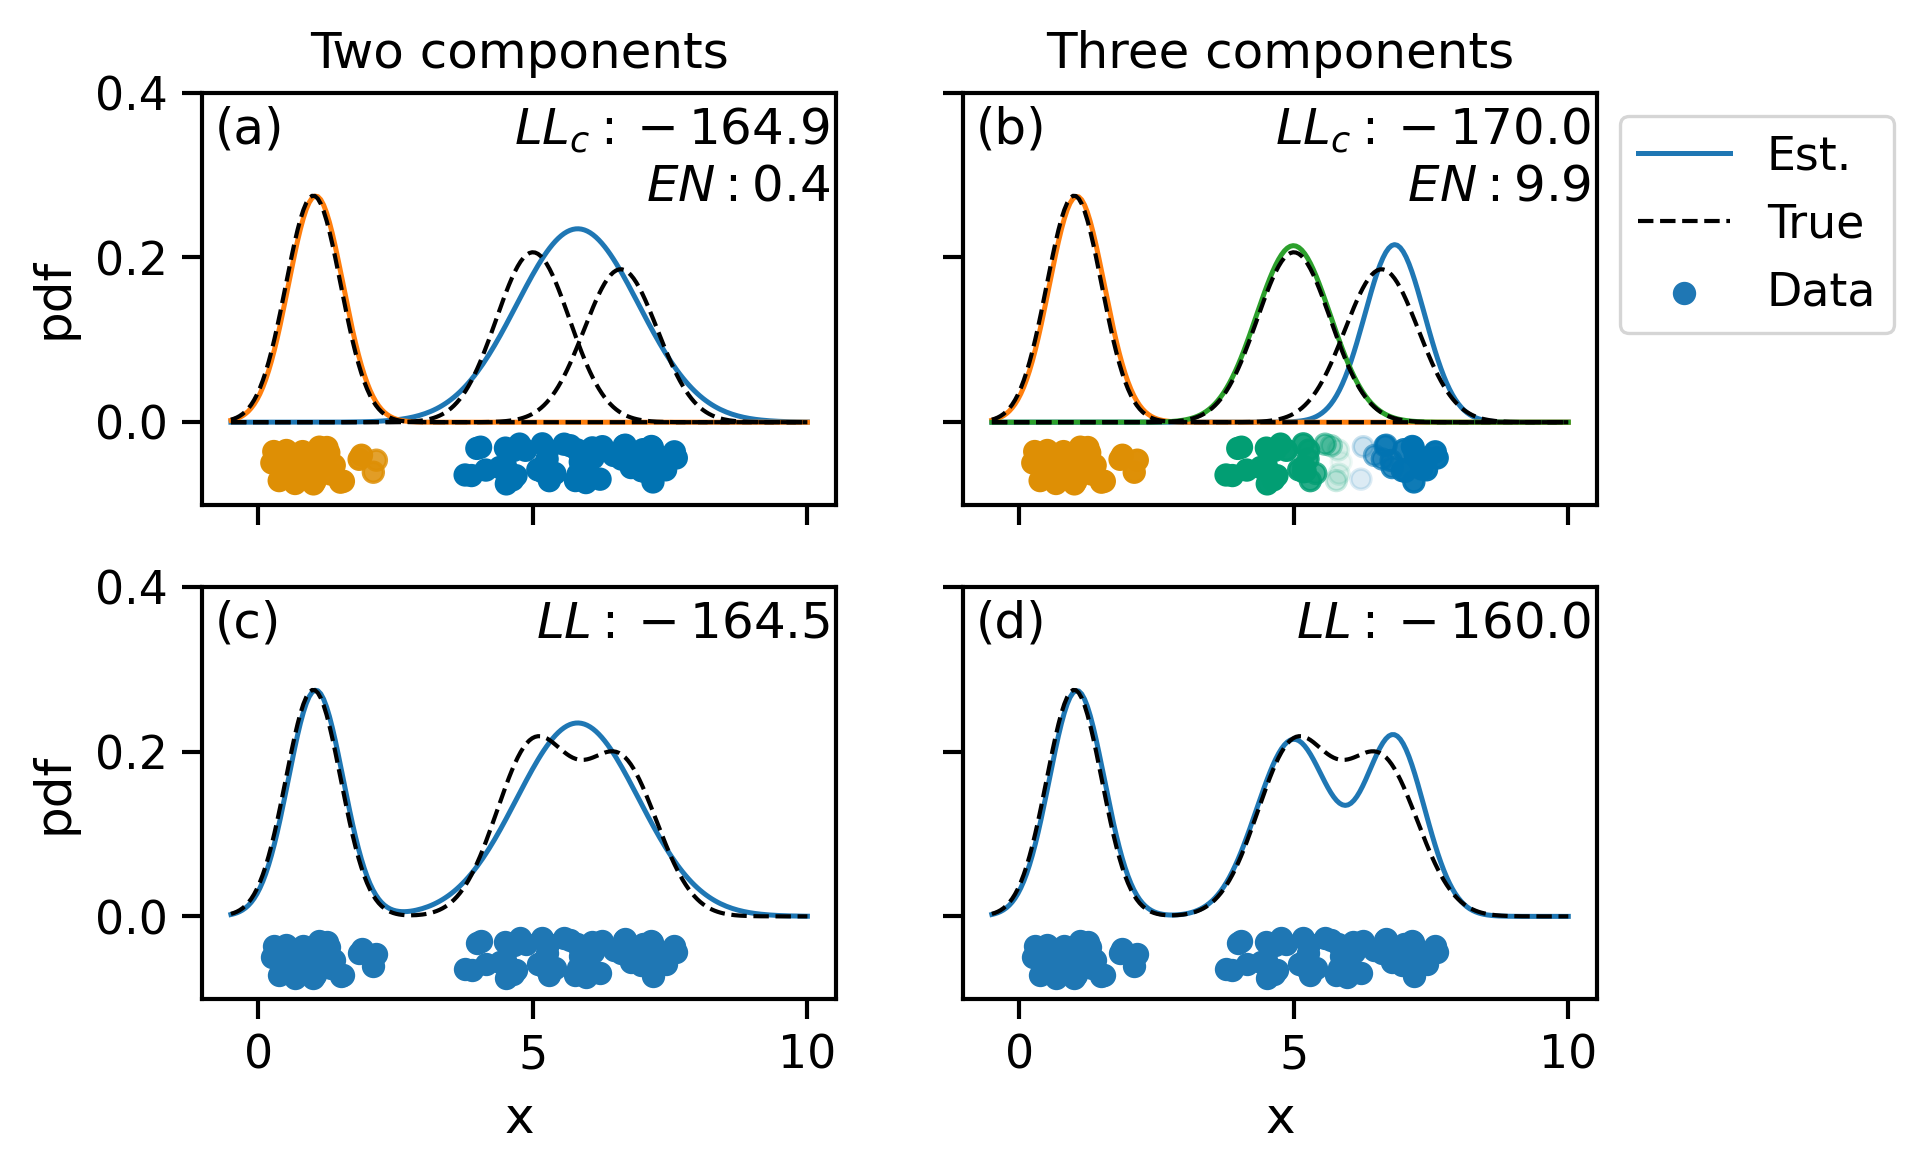
\includegraphics[width=0.8\textwidth]{chapters/hmm_selection/figures/class_like_explainer.png}
    \label{fig:hmm_class_lik_explainer}
\end{figure}

A related but different approach comes from  considering HMMs as a type of finite mixture model. \cite{mclachlanFiniteMixtureModels2000} Finite mixture models, such as Gaussian mixtures \cite{reynolds2009gaussian}, are used for two purposes (a) modelling the density of observations and (b) classifying observations into meaningful groups.\cite{mclachlan1988mixture} This is demonstrated in figure \ref{fig:hmm_class_lik_explainer} which shows $N = \num{87}$ random draws (coloured discs) from three normal distributions (black dashed lines). In panel (a) a two component Gaussian mixture model (GMM) has been estimated. To do this, the data $\{s_{1}, \ldots, s_{\mathrm{N}}\}$ were modelled as arising from the weighted sum of two normal distributions: $s \sim \pi_{1}\mathcal{N}\left(\mu_{1}, \sigma_{1}^{2}\right) +  \pi_{2}\mathcal{N}\left(\mu_{2}, \sigma_{2}^{2}\right)$. The values of the parameters $\theta = (\mu_{1}, \mu_{2}, \sigma_{1}, \sigma_{2}, \pi_{1}, \pi_{2})$ were chosen to maximise the log likelihood $\log{\mathcal{L}(\theta | \{s_{i}\})} = \mathbb{P}(\{s_{i}\}|\theta)$.  The coloured lines show the estimated normal distributions and the observations have been classified and coloured as arising from either one of the normal distributions. To classify the observations, the posterior probability of an  observation, $s_{i}$, arising from component $j$ (the distribution with parameters $\mu_{1}, \sigma_{1}$), was calculated: $M_{i,j}=\mathbb{P}(s_{i} \in \text{component }j |s_{i})$ for each value of $j$. The observations were assigned to the component with the highest value of $M_{i, j}$. This is known as the maximum a posteriori (MAP) assignment. In panel (c) the same model is shown but the total probability density (the sum of the probability density functions) is shown along with the log likelihood ($LL$). The same thing is repeated for a three component model in panels (b) and (d). So panels (a) and (b) reflect on GMMs as a method of classification, while panels (c) and (d) reflect on GMMs as a method of density estimation. 

How can the two models be evaluated?  For the purposes of density estimation, the estimated density of the three component model (panel (d) blue line) captures the bimodal distribution of the cluster of observations $x \in [4, 8]$ better than the two component model. This is to be expected as the data was generated from a three component mixture and the log likelihood reflects this: $LL=\num{-164}$ vs. $LL=\num{-160}$ for the two and three component models respectively. From a classification perspective the situation is reversed. For both models, the cluster of data around $x\simeq 1$ is unambiguously classified as belonging to a single component. For the two component model this is also true of the observations $x  \in [4, 8]$. However, for the three component model, the  distributions of the second and third components overlap in the small region around $x\simeq 5.8$. This means the posterior probabilities for belonging to either component, $M_{i, 2},\ M_{i, 3}$,  for the observations in this region will be similar. Therefore, it is not possible to unambiguously assign observations to either component $j=2$ or $j=3$. This is reflected in the log \emph{classification} likelihood, $LL_{c}$ which for the three component model is smaller than the two component model: $LL_{c}=\num{-170}$ vs. $LL_{c} = \num{-165}$. The log classification likelihood and the log likelihood are related by $LL = LL_{c} - EN$, where $EN$ is the classification entropy.\cite{hathaway1986another}  The entropy of an observation, $s_i$, is the information entropy  $H_i = \sum_{j}^{g}M_{i,j}\log{M_{i,j}}$  and measures the uncertainty with which the observation can be assigned to a given component.\cite{mackay2003information} The classification entropy is the sum of the individual entropies over the observations.\cite{mclachlanFiniteMixtureModels2000} So although the three component model has a higher \emph{likelihood} than the two component model, it has a lower \emph{classification likelihood} because it cannot assign all the observations with certainty to each component. 

The relationship between the Gaussian mixture model described above and a hidden Markov model is straightforward. The observations in a continuous state space $s_{i} \in \mathbb{R}$ map to the discrete microstate trajectories, $s_{t} \in \mathbb{Z}$; the components are the hidden states $h_{t}$; the distribution parameters $\mu_{i}, \sigma_{i}$ are the rows of the emission matrix, $E_{i, \cdot}$; and the mixing proportions are are stationary distribution $\bm{\pi}$. Considering HMMs as a coarse-graining procedure means they are aligned the second purpose of mixture models: \emph{classifying observations into meaningful groups}, where the `meaningful groups' are the system's metastable states. The classification likelihood is also known as the complete-data likelihood because the classification procedure adds in a new variable, the identity of the component associated with each observation. The complete-data likelihood takes both the observation \emph{and} the component variable into account.\cite{mclachlan1988mixture} To emphasise the difference between the likelihood and the complete-data likelihood, the former will be referred to as the observed likelihood.  

Using the complete-data likelihood may therefore be a more natural way to assess a HMM for coarse graining MSMs. Indeed a low value of the classification entropy indicate that the emission distributions do not overlap - one of the assumptions under which HMMs are valid representations of PMMs. However, although the relative values of $LL$ and $LL_{c}$ for the two models in the above example demonstrate the difference between the classification and density estimation paradigms for mixture models, using them to assess the number of components is difficult. For a thorough discussion on the reasons for this see section 6.4 of \cite{mclachlanFiniteMixtureModels2000} but briefly it arises from the fact that one can always estimate a model where the stationary distribution of one hidden states is zero thus making a smaller model (with fewer hidden states) potentially indistinguishable from the larger model. The Bayes factor approach is to integrate out all potential values of $\theta$ from the likelihood as described above. This is also possible with classification likelihood \cite{latoucheBayesianMethodsGraph2010} although to the best knowledge of the author of this thesis, this has not been done for reversible hidden Markov models. The two approaches for HMMs may be concisely compared as follows. The integrated observed likelihood measures the evidence for the HMM provided by the observed microstate trajectories, while the integrated complete-data likelihood measures the evidence for the model  given by the observed microstates and the given hidden states. 

Although the integrated observed and complete-data likelihoods are Bayesian quantities which generally require numerical approximation, analytic approximations exist which extend their use to models estimated using maximum likelihood. \cite{kassBayesFactors1995}\cite{mclachlanFiniteMixtureModels2000} The most widely used approximation to the integrated observed likelihood is the Schwarz criterion \cite{schwarzEstimatingDimensionModel1978a}, which up to an arbitrary factor is the Bayesian information criterion, BIC. The BIC was derived in the context of linear models and the approximations used are not valid in the finite mixture context, however there are other theoretical and practical reasons in favour of their use. \cite{fraley1998many} The analogue of the BIC for the integrated classification likelihood is the integrated complete-data likelihood criterion, ICL, \cite{biernackiAssessingMixtureModel2000a}.  The derivation of the ICL makes use of the same approximations as the BIC and so shares its drawbacks, however, in simulation experiments (for both HMMs and mixture models in general) it has performed well. \cite{mclachlanFiniteMixtureModels2000}\cite{celeuxSelectingHiddenMarkov2008}\cite{biernackiAssessingMixtureModel2000a}

Another type of approach to selecting the number of hidden states in maximum likelihood HMM models is via minimization of the Kullback-Liebler (KL) divergence \cite{kullbackInformationSufficiency1951}. The KL divergence  measures the difference between the modelled distribution and the true distribution. Two criteria which minimize this value are the Akaike-information criterion (AIC) \cite{akaikeInformationTheoryExtension1998} and the cross-validated log-likelihood, \cite{celeuxSelectingHiddenMarkov2008} CVLL. Although in both cases the likelihood used is the observed data likelihood and so neither of these criteria take into account the hidden state structure in a manner similar to the ICL. 

The benefits of the information criteria, BIC, ICL, and AIC, are that they require  very little extra calculation once a maximum likelihood HMM has been estimated. This is important as the search space of different models and number of hidden states may be large, rendering a more detailed Bayesian analysis for every potential model infeasible. However these methods have drawbacks both practical, mathematical and inferential. One potentially unrealistic assumption is that model selection using the AIC and BIC (and by analogy, the ICL) requires that the model representing the true data generating process must be in the model under consideration \cite{ripley_1996}. As HMMs are approximation to the true dynamics, this may be an unreasonable assumption. The reasons for this differ between the AIC and BIC however - for the Bayesian argument for the BIC see chapter 6 of \cite{bernardo2007bayesian}. In addition, the BIC and ICL criteria use approximations that are only valid under certain technical regularity conditions.\cite{mclachlanFiniteMixtureModels2000} These are the same difficulties which arise for  model selection using $LL$ and $LL_{c}$.  The benefit of the CVLL  is that it is conceptually simple but practically  one must estimate many HMMs to evaluate the number of hidden states. Other criteria exist for selecting the number of hidden states, for example the Penalised Marginal Likelihood criterion (PML) \cite{gassiatLikelihoodRatioInequalities2002} for MLE HMMs which circumvents some of the issues alluded to for the BIC, as well as a range of Bayesian model selection techniques \cite{gelmanBayesianDataAnalysis2014}\cite{bernardo2007bayesian}, however these are not considered here. 

Previous work \cite{mcgibbonStatisticalModelSelection2014a} evaluated the use of the AIC, BIC and CVLL for selecting the number of microstates in Markov state models. Choosing MSM parameters has since been superseded by the variational approach to learning Markov process (see chapter \ref{chap:msm}). This chapter builds on this work and investigates the use of the BIC, ICL, AIC, and CVLL to identify the number of hidden states in a HMM used for coarse-graining a MSM. It is similar to the investigation of these criteria in \cite{celeuxSelectingHiddenMarkov2008} but uses data simulated from the four well Prinz potential. This is an interesting extension of typical simulation benchmarks because the dynamics of the Prinz potential is (a) already approximately Markovian in the observed states and (b) the dynamics does not derive from an existing HMM (unlike most simulation studies which use data derived from an HMM process). The results of this chapter will be applied to the case of coarse graining MSMs of AADH in chapter \ref{chap:aadh}.  The structure of this chapter is as follows: in section \ref{sec:hmm_methods} the Prinz potential and the model selection criteria will be explained; section \ref{sec:hmm_results} discusses the results and section \ref{sec:hmm_conclusions} discusses the conclusions and limitations.

\section{Methods} \label{sec:hmm_methods}
\subsection{Prinz potential}
\begin{figure}[p]
    \centering
    \mycaption[The Prinz potential]{\textsc{The Prinz potential}. Panel (a) shows the potential $V(x)$, in blue and the stationary distribution, $\pi(x)$ in orange. Panel (b) shows the exact ratio of successive eigenvalues resolvable with a MSM with $\tau=5$. Panel (c) shows the exact ratio of successive timescales. Panel (d) shows the estimated implied timescales, $\hat{t}_{i}$, as coloured dashed lines with \SI{95}{\percent} credible intervals estimated using trajectories sampled from the potential using a Bayesian HMM with $1000$ draws from the posterior. The exact values, $t_{i}$, are shown as similarly coloured solid lines. The values of $\tau = 5, 8, 15, 65, 130$ used in the model selection experiments are shown as vertical black lines.}
    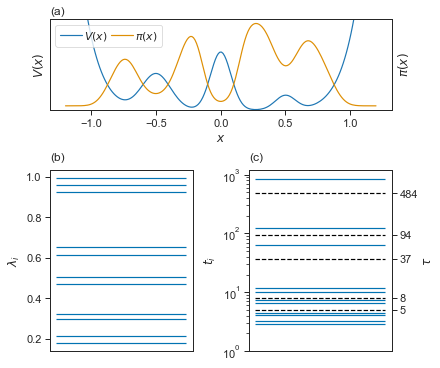
\includegraphics[width=0.8\textwidth]{chapters/hmm_selection/figures/prinz_pot.png}
    \label{fig:prinz_pot}
\end{figure}

The Prinz potential \cite{prinzMarkovModelsMolecular2011} is shown in figure \ref{fig:prinz_pot}.  Panel (a) shows the four well potential, $V(x)$, in blue and the stationary distribution, $\pi(x)$, showing the four metastable states, in orange. Panel (b) show the  ratio of successive eigenvalues resolvable by a  MSM with $\tau=5$. The large gap between the fourth and fifth eigenvalues implies four metastable states. Panel (c) shows the exact ratio of implied timescales. The implied timescales show a large gap between the second and third implied timescale. From this potential \num{100} independent trajectories were sampled, initialized from random draws from the stationary distribution, discretised into \num{410} microstates and used as data for estimating the HMMs in this work. The number of microstates was chosen as the square root of the number of observations, inline with the heuristic in \cite{husicWardClusteringImproves2017a}. See appendix \ref{app:hmm} for full details of the Prinz potential and simulation details. Panel (d) shows the mean implied timescales and \SI{95}{\percent} credible intervals as a function of the Markov lag time estimated with a Bayesian HMM. The exact timescales are also shown as solid lines. The estimated HMMs capture the exact times to within statistical uncertainty for all values of $\tau$ except for $t_{4}$ for $\tau < 8$. The number of hidden states used in these HMMs was determined by the lag time and the exact timescales of the full Prinz transfer operator (see table \ref{tab:prinz_its_exact}). For example for $\tau = 130$ only $t_2 = 844$ is resolvable so a two hidden state HMM was used. The time and rate units used throughout this chapter are in terms of the time-step used to integrate the equations of motion, $\Delta t = 0.001$, and the distance units are arbitrary, see section \ref{sec:app_hmm_prinz}.

\subsection{Model selection criteria}

In the following sections, the likelihood, $\mathcal{L}$, of the HMM parameters will feature heavily and so is repeated here for convenience \cite{noeProjectedHiddenMarkov2013a}: 

\begin{equation}\label{eqn:obs_lik_full}
\begin{split}
    \mathcal{L}\left(\tilde{\mathbf{T}}, \mathbf{E}| \{s_t\}\right) & = \mathbb{P}\left(\{s_t\} | \tilde{\mathbf{T}}, \mathbf{E}\right) \\
    & = \sum_{\substack{\{h_t\} \in \\ \text{all paths}}} \tilde{\pi}_{h_{0}}E_{h_{0},s_{0}}\prod_{t=1}^{t_{max}}\tilde{T}_{h_{t-1}, h_t}E_{h_t, s_t}    
\end{split}
\end{equation}
This is the likelihood of the parameters of the transition matrix and emission matrix ($\tilde{\mathbf{T}}, \mathbf{E}$ respectively) given the trajectory of observed states $\{s_t\}$. The multiplicand represents the probability of observing Markovian transition between hidden states (the $\tilde{T}_{h_{t-1}, h_{t}}$ term) and then  observing the observed states (the $E_{h_t, s_t}$ term). The summand represents summing the probability over all possible combinations (paths) of hidden states, while $\tilde{\pi}_{h_{0}}E_{ h_{0}, s_{0}}$ is the probability of the initial hidden state/observed state pair. This summation is infeasible for even small numbers of hidden states and trajectory lengths (e.g. for $2$ hidden states and a trajectory of $100$ frames, there are approximately $10^{30}$ potential paths). The Baum-Welch algorithm \cite{rabinerTutorialHiddenMarkov1989} was developed to maximize the likelihood through expectation maximisation. An outline of the Baum-Welch algorithm can be found in algorithm \ref{alg:baum_welch}, while the full details for maximum likelihood HMMs can be found in \cite{noeProjectedHiddenMarkov2013a}. The maximum likelihood estimates of the parameters will be denoted $\hat{\theta}$, so the maximum of the likelihood function will be denoted $\mathcal{L}\left(\hat{\theta}|\{s_t\}\right)$. 

Selecting the number of hidden states using CVLL and the AIC both minimize the \emph{Kullback-Leibler} divergence, $D_{\mathrm{KL}}(p||q)$.  \cite{mclachlanFiniteMixtureModels2000} This is a measure of the difference between a given probability distribution, $p(s)$ and a reference distribution, $q(s)$: 

\begin{equation}\label{eqn:kl_div}
\begin{split}
    D_{\mathrm{KL}}\left(p\mid | q\right) & = \int q(s) \log{\left(\frac{ q(s) }{p(s)}  \right)} \mathrm{d}s \\ 
    & = \int q(s) \log{\left(q(s)\right)}\mathrm{d}s - \int q(s)\log{\left(p(s)\right)} \mathrm{d}s
\end{split}
\end{equation}
When the two distributions are the same $D_{\mathrm{KL}} = 0$. The first term is the average information of $q(s)$, also known as the information entropy. \cite{mackay2003information} This is continuous analogue of the information entropy discussed in the introduction, albeit for a different distribution. The second term is average information of $p(s)$ but averaged over reference distribution.\cite{mackay2003information} In the context of model selection, $p(s)$, is taken to be the modelled distribution $\mathbb{P}(\{s_t\}|\hat{\theta})$ and $q(s)$ is the unknown true distribution. As only the latter term is dependent on the modelling choices and  $D_{\mathrm{KL}} \ge 0$ (Jensen's inequality \cite{mackay2003information}) maximizing this term will lead to the model closest to the true distribution.  

The AIC approximates the second term in equation \ref{eqn:kl_div} and is defined as: \cite{akaikeInformationTheoryExtension1998}
\begin{equation}\label{eqn:aic}
    \operatorname{AIC} = -2\log{\left(L\left(\hat{\theta}|\{s_t\}\right)\right)} + 2d
\end{equation}
where $d$ is the number of degrees of freedom of the model. For a reversible Markov transition matrix with $g$ states this is: $d = \sfrac{1}{2}g(g-1) + (g-1)$. \cite{trendelkamp-schroerEstimationUncertaintyReversible2015b} The emission distribution adds $g(n-1)$, as for every hidden state $g$ there are $n$ probabilities which must sum to $1$ giving $n-1$ degrees of freedom per hidden state. So the total degrees of freedom for a reversible HMM is:
\begin{equation}\label{eqn:hmm_dof}
    d = \sfrac{1}{2}g(g-1) + (g-1) + g(n-1). 
\end{equation}
The derivation of the AIC starts by approximating the true distribution, $q(s)$, with the distribution over $s$ estimated from the data. This gives rise to the $\log{L\left(\hat{\theta}|\{s_t\} \right)}$ term.\cite{mclachlanFiniteMixtureModels2000}  This will naturally over-fit to the data and the $d$ term attempts to account for this. $d$ is only equal to the degrees of freedom of the model under the assumption that the true model is under consideration in the model selection procedure \cite{ripley_1996}.  The factor of $-2$ is there to make an equivalence with Mallows $C_p$ \cite{friedman2001elements} although this doesn't affect the final results. The selected model is the one which has the smallest AIC. 

Instead of approximating $q(s)$ with $\mathcal{L}\left(\hat{\theta}|\{s_t\}\right)$ and making a bias correction, cross-validation can be used to approximate the second term of equation \ref{eqn:kl_div}.\cite{celeuxSelectingHiddenMarkov2008} In this work, the CVLL was calculated in the following way (note, this is different from the procedure in \cite{celeuxSelectingHiddenMarkov2008}): 
\begin{enumerate}
    \item The observed trajectories were split into $N = 10$ training $\{s_t\}^{i}$ and test $\{s_t\}^{-i}$, $i = 1, ..., N$ sets using 50:50 shuffle-split (algorithm \ref{alg:shuffle_split}). 
    \item For each $i$, an HMM was estimated using the training data $\{s_t\}^{i}$. 
    \item Calculate the log-likelihood of the training parameters using the test data,  $\log{\left(\mathcal{L}\left(\hat{\theta}^{i}\middle|\{s_t\}^{-i}\right)\right)}$, with the forward part of the Baum-Welch algorithm (algorithm \ref{alg:baum_welch}). 
    \item The CVLL is the average over the splits: 
    \begin{equation}
        \operatorname{CVLL} = \frac{1}{N}\sum_{i}^{N}\log{\left(\mathcal{L}\left(\hat{\theta}^{i} \middle | \{s\}^{-i}\right)\right)}
    \end{equation}
\end{enumerate}
There are two potential points of failure in this procedure. First, the HMM may fail to converge on a given fold. Second, the `forward' part of the Baum-Welch algorithm may fail to give a finite estimate for the log-likelihood. If either of these failures occurred, the CVLL value for that number of hidden states was considered invalid. 

The BIC comes from consideration of the integrated observed likelihood, $\mathbb{P}\left(\{s_t\}\right)$ used in the definition of the Bayes factor: 
\begin{equation}\label{eqn:obs_lik_int}
       \mathbb{P}\left(\{s_t\}|M\right) = \int \mathbb{P}\left(\{s_t\}\middle|\theta \right)\mathbb{P}\left(\theta \middle | M\right) \mathrm{d}\theta,
\end{equation}
where $\mathbb{P}(\theta)$ is the prior distribution over the HMM parameters for a given model specification. The integrated likelihood selects the model with the greatest evidence for the observed states, i.e., the model with the highest posterior probability, given the observed states and taking into account the increased flexibility of more complex models. \cite{mackay2003information}\cite{kassBayesFactors1995} The BIC is an approximation to the logarithm of equation \ref{eqn:obs_lik_int} and is given by:\cite{schwarzEstimatingDimensionModel1978a}
\begin{equation}\label{eqn:bic}
    \operatorname{BIC} = -2\log{\left(\mathcal{L}\left(\hat{\theta}\middle| \{s_t\}\right)\right)} + d\log{\left(N_{\mathrm{obs}}\right)}
\end{equation}
where $d$ is the degrees of freedom and $N_{\mathbf{obs}}$ is the number of observations.  The difference in BIC between two models, $\mathrm{BIC}_{1}-\mathrm{BIC}_{2}$ is an approximation to the log of the Bayes factor, the selected model is then the one with the smallest BIC.  The derivation of the BIC proceeds by expanding the log of the integrand in equation \ref{eqn:obs_lik_int},  $\log{\left(\mathbb{P}\left(\{s_{t}\}\middle |\theta \right)\right)}$ in a Taylor series about $\hat{\theta}$ up to second order. The regularity conditions alluded to in the introduction amount to the ability to safely ignore the higher order terms in this expansion.\cite{mclachlanFiniteMixtureModels2000}

The derivation of the ICL follows an analogous path to the BIC but takes as its starting point the integrated complete-data likelihood: 
\begin{equation}\label{eqn:class_lik_int}
    \mathbb{P}\left(\{(s_t, h_t)\}\middle | M \right) = \int \mathbb{P}\left(\{(s_{t}, h_{t})\}\middle |\theta \right)\mathbb{P}\left(\theta\middle | M\right) \mathrm{d}\theta
\end{equation}
The integrated complete likelihood selects the model with the greatest evidence for the observed states \emph{and} the hidden states. As the hidden states are not observed they are taken to be MAP assigned values: $h_t = \argmax_{j} M_{s_{t}, j}$. The ICL is an approximation to $\log{\left(\mathbb{P}(\{(s_t, \hat{h}_t)\}\middle | M \right)}$ and is given by:\cite{biernackiAssessingMixtureModel2000a}
\begin{equation}\label{eqn:icl}
\begin{split}
        \operatorname{ICL} &= -2\log{\left(L\left(\hat{\theta}\middle|\{s_t\}\right)\right)} + d\log{\left(N_{\mathrm{obs}}\right)} +2\cdot EN\left(\mathbf{M}\right)     \\
        & = \operatorname{BIC} + 2\cdot EN\left(\mathbf{M}\right)
\end{split}
\end{equation}

The $EN$ term  is classification entropy given by:\cite{biernackiAssessingMixtureModel2000a} 
\begin{equation}
\begin{split}
     EN\left(\mathbf{M}\right) & = \sum_{t}^{N_{\mathrm{T}}}(-1)\sum_{j}^{g} M_{s_{t}, j}\log{\left(M_{s_{t}, j}\right)}  \\ 
     & =\sum_{t}^{N_{\mathrm{T}}} H\left(s_{t}; \mathbf{M}\right)
\end{split}
\end{equation}
Here $\mathbf{M}$ is the membership matrix $M_{i,j}= \mathbb{P}(h=j|s=i)$ and $H$ is the information entropy $H\left(s_{t};\mathbf{M}\right) = -\sum_{j} M_{s_{t}, j}\log{\left(M_{s_t, j}\right)}$. This entropy quantifies the uncertainty with which the model assigns the given observed state to a hidden state. For example in a two hidden state system, given an observed state which could belong in hidden state 1 with probability \SI{50}{\percent} or in hidden state 2 with probability \SI{50}{\percent}, then the entropy for that observation is:
\begin{equation}
\begin{split}
    H\left(s; \mathbf{M}\right) & =  -\sum_{j} M_{s_{t}, j}\log{\left(M_{s_t, j}\right)} \\
    & = -\sfrac{1}{2}\log{\left(\sfrac{1}{2}\right)} - \sfrac{1}{2}\log{\left(\sfrac{1}{2}\right)} \\
    & = \log{\left(2\right)}
\end{split}
\end{equation}
 
\subsection{Criteria calculation details}\label{sec:hmm_details}
There are a number of practical details in calculating the information criteria which need to be addressed. 

The number of observations, $N_{\mathrm{obs}}$, needed for the BIC and ICL, was calculated as the number of pairs of observations which go into the count matrix. Using the sliding window count method this is:
\begin{equation}
    N_{\mathrm{obs}} = N_{\mathrm{traj}}\cdot\frac{(N_{\mathrm{T}} - \tau)}{\Delta t}
\end{equation}
where $N_{\mathrm{traj}}$ is the number of trajectories, $N_{\mathrm{T}}$ is the length of each trajectory, $\tau$ is the Markov lag time and  $\Delta t$ is the trajectory time-step. The total number of frames is $N_{\mathrm{frames}} = N_{\mathrm{traj}}\cdot N_{\mathrm{T}} /\Delta t$

The classification entropy was calculated using the hidden state probabilities calculated in the final iteration of the Baum-Welch (B-W) algorithm (algorithm \ref{alg:baum_welch}): 
\begin{enumerate}
    \item For each observed state in a trajectory, $s_t$, the conditional probability, $\gamma_{i}(t)=\mathbb{P}\left(h_{t}=i \mid s_t, \theta\right)$, was extracted from the final iteration of `update' part of the B-W algorithm. 
    \item The entropy was calculated for each frame of the trajectory,  $H(t)=-\sum_{i}\gamma_{i}(t)\log{\left(\gamma_{i}(t)\right)}$ and then summed over the $N_{\mathrm{T}}$ frames of a trajectory and then over the $N_{\mathrm{traj}}$ trajectories: $EN = \sum^{N_{\mathrm{traj}}} \sum_{t}^{N_{\mathrm{T}}} H(t)$.
    \item $N$ was scaled by a factor of $N_{\mathrm{obs}}/N_{\mathrm{frames}}$ to account for the fact that an observation is a pair of states $(s_{t}, s_{t+\tau})$.
\end{enumerate}
A second method was available, which in principle should give the same answer but which in practice diverged by up to a factor of three from the above method. The entropy was calculated using the membership matrix, itself calculated from the emission matrix, $\mathbf{E}$, and the stationary distributions of the hidden $\widetilde{\bm{\pi}}$ and observed $\bm{\pi}$ states: 
\begin{equation}\label{eqn:M_vs_E}
    M_{j,i} = E_{i,j}\frac{\widetilde{\pi}_{i}}{\pi_{j}}
\end{equation}
where $i$ labels the $g$ hidden states and $j$ labels the $n$ observed states. The entropy was calculated using $\mathbf{M}$ as: 
\begin{equation}\label{eqn:ent_v2}
    \mathrm{EN} = N_{\mathrm{obs}}\sum^{n}_{j}\pi_{j}\sum^{g}_{i} M_{ji}\log{\left(M_{ji}\right)}
\end{equation}
The reason for the difference was due to error accumulated in the values of  $\mathbf{M}$ from equation \ref{eqn:M_vs_E}. This was due to noise in the poorly sampled observed states, see section \ref{sec:app_membership_errors} and figure \ref{fig:membership_error}. However, in situations when the largest reversible connected set of hidden states is smaller than total number of hidden states, the values of $\gamma$ would need re-normalizing. In this case (in particular in chapter \ref{chap:aadh}) the second method will be more convenient. 

\subsection{Model selection experiment}
The model selection criteria were used to select the optimum number of hidden states in a maximum likelihood HMM, using the discrete trajectories sampled from the Prinz potential. Five different values of the Markov lag time were used: $\tau=5, 8, 15, 65, 130$. These values were chosen because they resolve, respectively $7, 5, 3, 2, 1$ implied timescales in the full MSM state space and as the top three of these timescales are dominant (figure \ref{fig:prinz_pot} panel (b)), these values of $\tau$ resolve $4, 4, 4, 3, 2$ metastable states  respectively.\cite{noeProjectedHiddenMarkov2013a} 

For each value of $\tau$ maximum likelihood HMMs were estimated with $g = 2 - 10$ hidden states. For each of the $45$ model specifications ($\tau$ and $g$) the model selection criteria were calculated  and the number of hidden states selected by each was compared to the true value. 

\section{Results and discussion}\label{sec:hmm_results}
\begin{table}
    \centering
    \mycaption[Hidden state selection results]{\textsc{Hidden state selection results}. The selected number of hidden states, $\hat{g}$, by the CVLL, AIC, BIC and ICL for each value of $\tau$. The true values, $g^{\mathrm{true}}$ are also shown. The asterisk highlights where $\hat{g}=g^{\mathrm{true}}$. The number in parentheses shows $\hat{g}-g^{\mathrm{true}}$. }
    \begin{tabular}{|c|c|c|c|c|c|}
    \hline
    $\tau$ & $g^{\mathrm{true}}$ & CVLL & AIC & BIC & ICL  \\
    \hline\hline
     $5$  & $4$ & $4^{*} (0)$  & $10 (6)$ & $10 (6)$ & $5 (1)$ \\
     $8$  & $4$ & $4^{*} (0)$ & $10 (6)$ & $8 (4)$  & $4^{*} (0)$  \\
     $15$ & $4$ & $4^{*} (0)$  & $9 (5)$ & $6 (2)$  & $4^{*} (0)$  \\
     $65 $& $3$ & $4 (1)$  & $5 (2)$  & $4 (1)$  & $3^{*} (0)$  \\
     $130$& $2$ & $4 (2)$  & $4 (2)$  & $3 (1)$  & $3 (1)$  \\
     \hline
    \end{tabular}
    \label{tab:prinz_criteria_results}
\end{table}

\begin{figure}
    \centering
    \mycaption[Hidden state selection criteria]{\textsc{Hidden state selection criteria}. Rows (a) - (e) show the selection criteria for HMMs with $\tau=5, 8, 15, 65, 130$ respectively. The best performing number of hidden states is indicated by an arrow. Column (i) shows the CVLL. Column (ii) shows the AIC. The log-likelihood term is shown in blue and the degrees of freedom penalty ($2d$) is shown in orange. Column (iii) shows the BIC. The penalty term $d\cdot\log{N_{obs}}$ is shown in green.  Column (iv) shows ICL. The classification entropy penalty term $2\cdot EN$ is shown in red. Missing values indicate the failure of the HMM to converge. All values have been scaled so the minimum value in each panel is $1$.}
    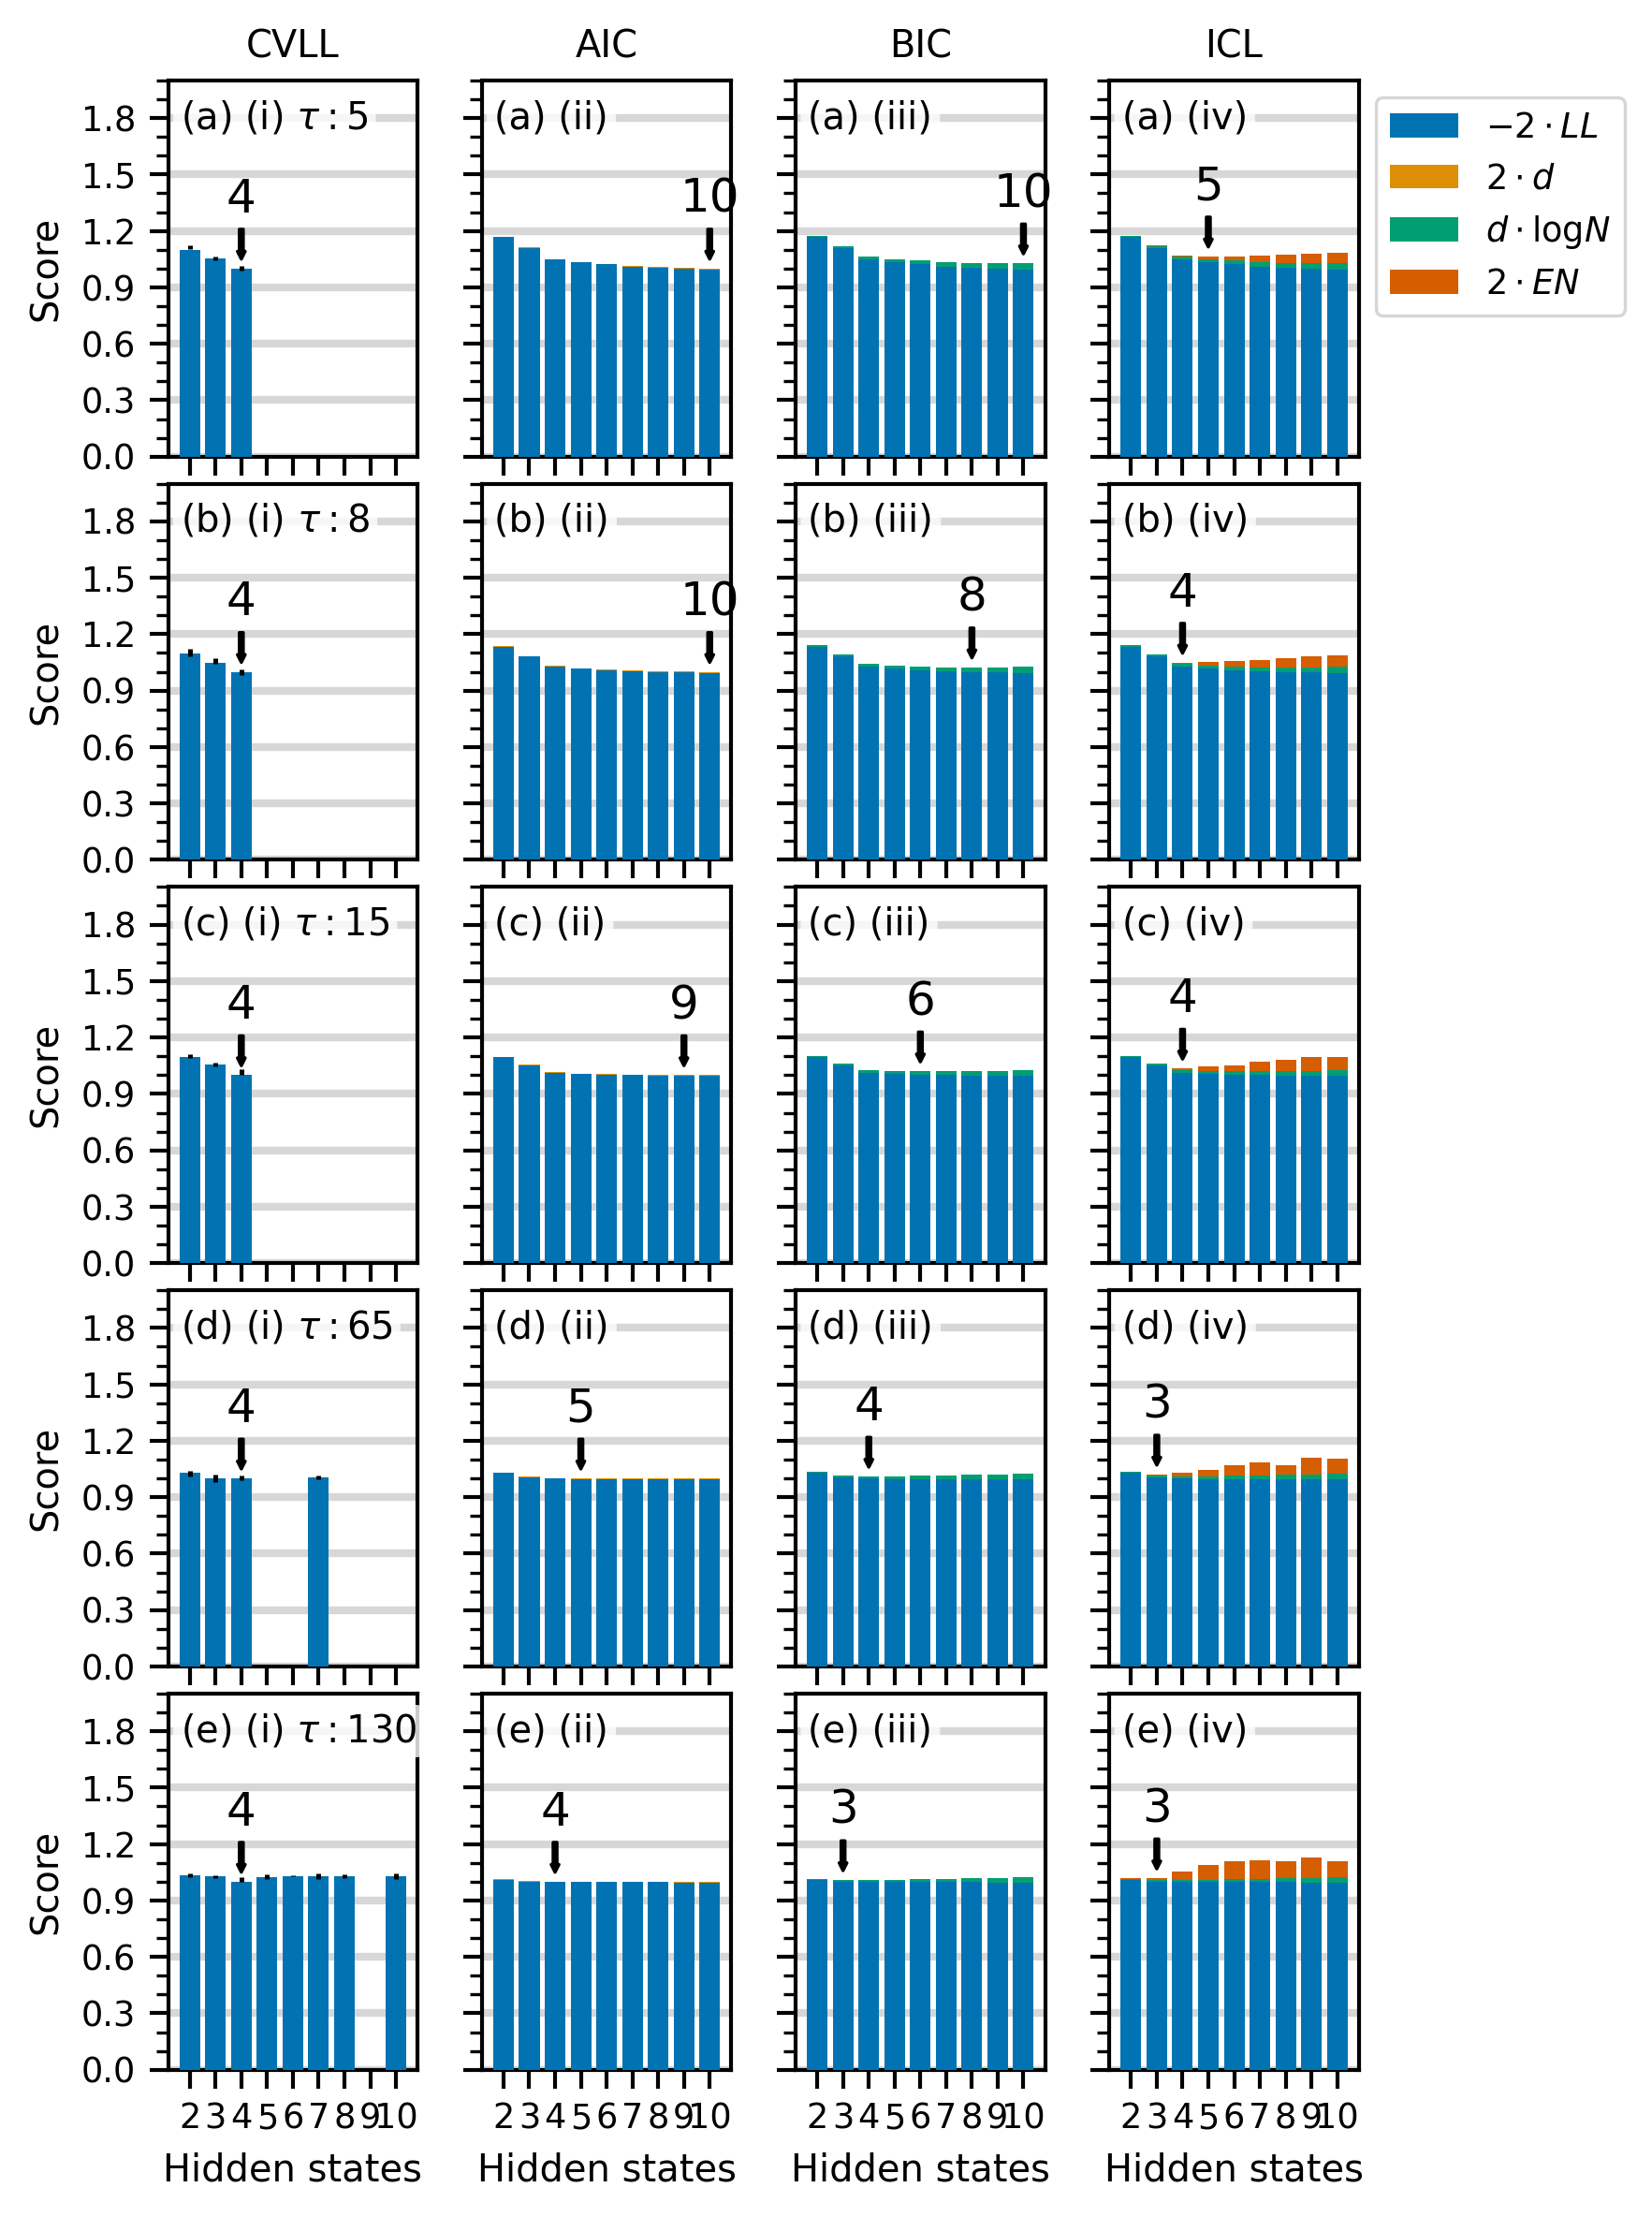
\includegraphics[width=0.75\textwidth]{chapters/hmm_selection/figures/prinz_h_state_selection.png}
    \label{fig:prinz_criteria_results}
\end{figure}

The selected number of hidden states using each criterion are shown in table \ref{tab:prinz_criteria_results} where the asterisk denotes when a criteria selects the correct number of hidden states. The relative values of the selection criteria are shown in figure \ref{fig:prinz_criteria_results}. Each row, (a) - (e), corresponds to models estimated with a  different value of the Markov lag time $\tau=5, 8, 15, 65, 130$. Each column, (i) - (iv), corresponds to the different model selection criteria, CVLL, AIC, BIC, and ICL. The minimum value of each criteria for each model is highlighted with an arrow indicating the selected number of hidden states, $\hat{g}$. The values are scaled so the value at the selected number of states the value of the criterion is equal to $1$.  The coloured bars show the contributions of the different parts of each score. The blue bars shows the log-likelihood terms of equations \ref{eqn:aic}, \ref{eqn:bic} and \ref{eqn:icl} i.e.  $-2\times \log{\left(\mathcal{L}\left(\hat{\theta}\middle |\{s_t\}\right)\right)}$. In the case of CVLL, the blue bars are the  cross-validated equivalent. The various penalty terms are shown in orange ($2d$ the AIC penalty), green ($d\log{N}$, the BIC penalty) and red ($2\cdot EN$, the classification entropy). 

The ICL performs best by correctly identifying the number of hidden states for $\tau=8, 15, 65$. It fails at $\tau=5$ where the hidden state dynamics are not quite Markovian (figure \ref{fig:prinz_pot} panel (d)). Although the selected value of $5$ is close to the true value of $4$, the ICL does not discriminate between $g=4 - 7$: their ICL values vary by less than \SI{1}{\percent}, as shown in figure \ref{fig:prinz_criteria_results} panel (a)(iv). The ICL also fails at $\tau=130$, however the minimum value of the ICL is similar to the value for the true number of hidden states, $g = 2$, and is significantly different to the values for $g \ge 4$,  as shown in panel (e)(iv). In this case the ICL does distinguish between two values of $g$ which include the true value on the one-hand, and the remaining values on the other. This behaviour is in contrast to the results in \cite{celeuxSelectingHiddenMarkov2008} in which the ICL correctly identified the number of hidden states for well separated emission distributions, and with large numbers of observations for less well separated distributions. However, for smaller numbers of observations and less well separated clusters, the ICL \emph{under-estimated} the number of hidden states. The ICL also under-estimated the number of clusters in the finite mixture context when the clusters are not well separated.\cite{biernackiAssessingMixtureModel2000a}

The CVLL correctly selects four states for $\tau = 5, 8, 15$, however this was due failure of the cross-validation to produce a finite answer on some of the cross-validation folds. For example, for $\tau=5$, at least one cross-validation fold did not estimate the out-of-sample log-likelihood for $g\ge 4$. The remaining values are shown in figure \ref{fig:prinz_criteria_results} column (i). This causes problems with interpretation as is it is not clear whether failure is due to the  inefficiency of the cross-validation procedure or whether the given number of hidden states really has zero out-of-sample likelihood. The former is more likely given that models estimated on \SI{100}{\percent} of the data do converge and give interpretable answers. Given the lack of convergence for many of the values of $g$ comparison with the literature is difficult. The results in \cite{celeuxSelectingHiddenMarkov2008} show that the CVLL behaves similarly to the ICL but with less discrimination between values of $g$ i.e., in repeated experiments the distribution of selected values of $g$ was wider. In contrast, the results for $\tau=130$ in figure \ref{fig:prinz_criteria_results} panel (e)(i) show the CVLL over-estimates the number of hidden states.  Given the poor performance of the CVLL in this experiment it will not be discussed further here. 

The AIC overestimates for every value of $\tau$ and as $\tau$ increases the values of the AIC discriminate less between each value of $g$: for $\tau = 130$ the AIC for all $g$ are within \SI{2}{\percent} of each other. This is in contrast to the results in   \cite{celeuxSelectingHiddenMarkov2008} which the AIC selected the correct or underestimated the value of $g$. However, in simulation studies for finite mixtures (without the Markovian dynamics of the hidden states) the AIC frequently over-estimated the number components. \cite{celeuxEntropyCriterionAssessing1996, soromenho1994comparing} The BIC also overestimates the number of hidden states for all values of $\tau$ but only by $1$ for $\tau=65$ and $130$. This is in contrast to the results in \cite{celeuxSelectingHiddenMarkov2008} for which the BIC behaved similarly to the ICL and either estimated correctly or under-estimated the number of hidden states.  In addition, for finite mixtures the BIC has also been shown to under-estimate the number of components.\cite{biernackiAssessingMixtureModel2000a} 

Although the AIC, BIC and ICL are derived from different starting points, they all take the form of the log-likelihood plus a penalty term, $b$:
\begin{equation}
    -2\log{\left(\mathcal{L}\left(\hat{\theta} \middle|\{s_t\}\right)\right)} + b
\end{equation}
The $b$ term in each case penalises the complexity of each model. The behaviour of these criteria can be understood in terms of the interplay between the likelihood and penalty terms. The log-likelihood, the blue bars in columns (ii)-(iv) of figure \ref{fig:prinz_criteria_results}, monotonically increases with $g$ for all values of $\tau$ (this is shown as a decrease due to the $-2$ in the definition of the criteria). This is most pronounced for small values of $\tau$ (compare panel (a)(ii) to (e)(ii)), and demonstrates both over-fitting and the HMMs ability to capture the fast relaxation processes of the Prinz dynamics. Consider the $g=10$ model selected by the AIC for $\tau=8$, figure \ref{fig:prinz_tau8_g10} (the results are similar for $\tau=5$). This figure shows the sign structure of the exact relaxation processes (panels (a) - (c)) and those estimated from the HMM (panels (d) - (f)). The HMM captures the sign structure of the second and fifth relaxation process,  panels (d) and (e), as they have associated timescales larger than $\tau$, ($t_{2}=844.4, t_{5} = 11.9 > \tau=8$) and are thus resolvable. The 10th estimated relaxation process (panel (f)) is clearly spurious - the estimated timescale $\hat{t}_{10} = 4.0$ is less than the lag time, $\tau$, and the sign structure does not match that of the exact process, panel (c). For larger values of $\tau$ and $\tau= 130$ in particular (figure \ref{fig:prinz_criteria_results} panel (e)(ii)), the likelihood remains constant. This is because there is only one resolvable true relaxation process and increasing the number of hidden states just over-fits to spurious relaxation processes[xxx still needs double checking].  

\begin{figure}
    \centering
    \mycaption[Comparison of estimated and true Prinz potential dynamics]{\textsc{Comparison of estimated and true Prinz potential dynamics}. The true Prinz potential are compared with a HMM with $\tau=8$ and $g=10$ hidden states. Panels (a) - (c) shows the sign structure of the 2nd, 5th and 10th right eigenvector of the Prinz potential ($\mathrm{sgn}[\Psi(x)]$, shaded area). The Prinz potential ($V(x)$, blue solid line) is shown for reference. The exact timescales are labelled on the top right as $t_{2/5/10}$.  Panels (d) - (f) show the sign structure of the hidden state relaxation processes, projected onto the observed states. The eigenvectors projected onto the observed state basis, $q_{2/5/10}(x) = \sum_{i} E_{i, x} \cdot \tilde{\Psi}_2(i)$ , are shown as dotted lines, the summands are shown as coloured lines. The shaded areas are $\mathrm{sgn}[q_{2/5/10}(x)]$. The estimated timescales are labelled on the top right as $\hat{t}_{2/5/10}$. }
    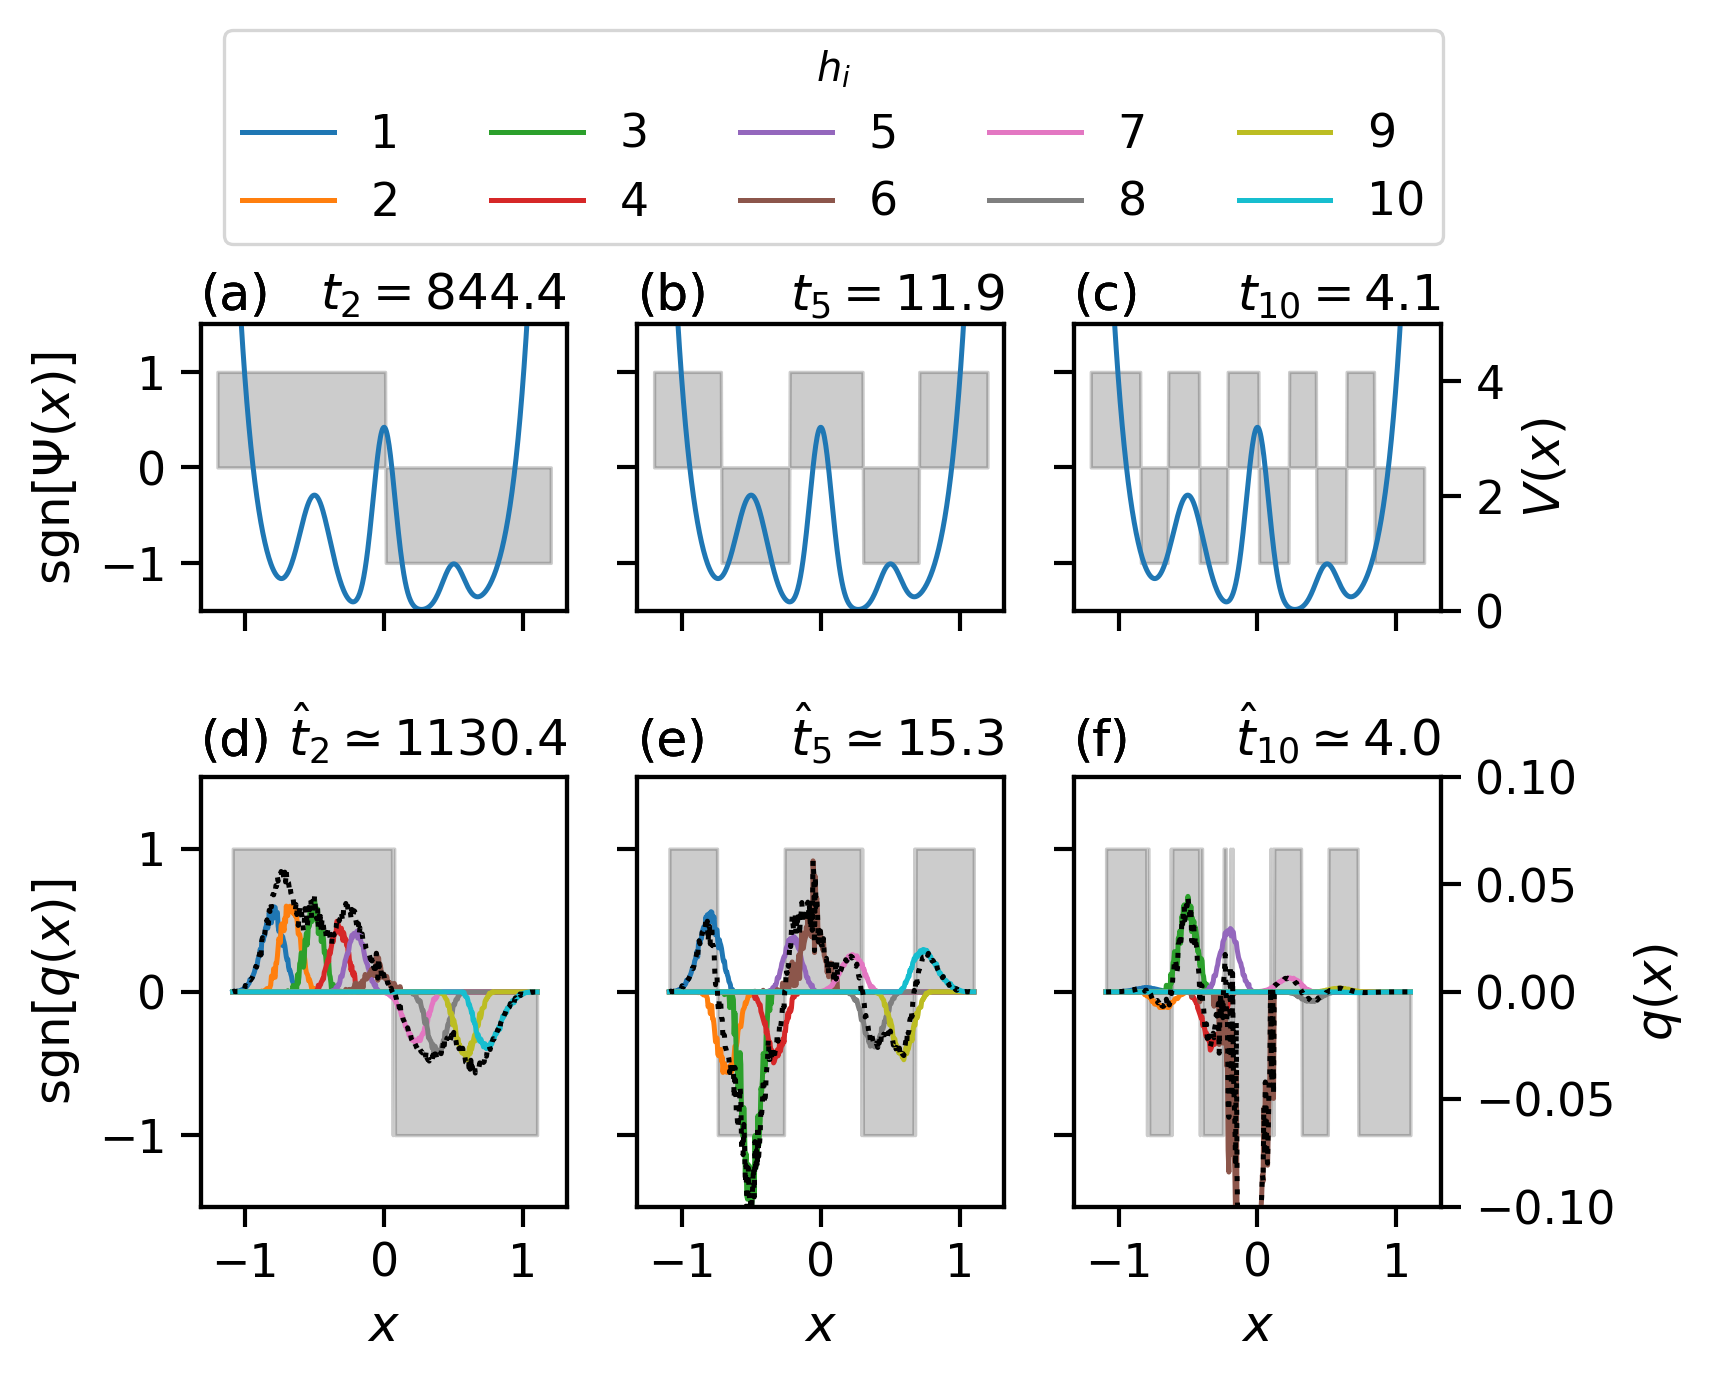
\includegraphics[width=0.8\textwidth]{chapters/hmm_selection/figures/hmm_tau_8_g_10.png}
    \label{fig:prinz_tau8_g10}
\end{figure}

The AIC the penalty term, $b=2d$ (orange bars in figure \ref{fig:prinz_criteria_results}, column (ii)), is there to correct the approximation of the KL divergence by log-likelihood. It increases proportional to $g^{2}$ (equation \ref{eqn:hmm_dof}) but only affects the selected $g$ for $\tau=15, 65, 130$ (figure \ref{fig:prinz_criteria_results} panels (c), (d) and (e)(ii)). The origin of the BIC penalty term, $b=d\log{N_{obs}}$ (green bars, column (iii)) is to correct the approximation of the integrated likelihood by the maximum log-likelihood. The BIC over-estimates the number of hidden states albeit by a smaller number than the AIC, due to the penalty term rising faster with $g$ by a factor $\log{N_{\mathrm{obs}}}/2$. As pointed out in \cite{mcgibbonStatisticalModelSelection2014a} when using the sliding window method for calculating the count matrix the value of $N_{\mathrm{obs}}$  will be overestimated. However, as the dynamics is approximately Markovian for $\tau > 5$ the difference between the sliding window and sample count methods (see section \label{sec:theory_count_mat}) will be negligible. 

\begin{figure}
    \centering
    \mycaption[The classification entropy of HMMs]{\textsc{The classification entropy of HMMs}. Panels (a)-(c) show the emission distributions of HMMs with $\tau=8$ and $g = 2, 4, 10$ respectively. Each coloured line represents the emission distribution, $E_{i, x}$,  of the hidden states, $i$. Panels (d) - (f) show the information entropy for observed state at $x$, weighted by the stationary distribution over the observed states: $\pi(x)H(x)$. The label shows the average classification entropy per observation $EN_{\mathrm{ave}} = \sum_{x}\pi(x)H(x)$.}
    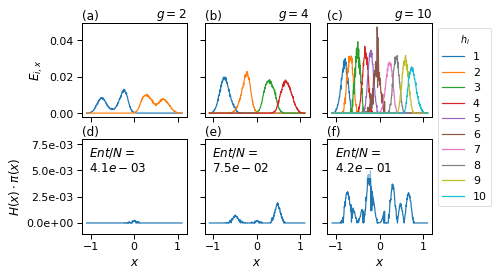
\includegraphics[width=0.8\textwidth]{chapters/hmm_selection/figures/prinz_entropy.png}
    \label{fig:prinz_ent}
\end{figure}

The ICL penalty term $b=d\log{N}+2\cdot EN$ corrects the approximation to the integrated complete-data likelihood by the log-likelihood. It is comprised of the BIC penalty term (green bars in figure \ref{fig:prinz_criteria_results}) and the entropy term (red bars). This is associated with increasing $g$ directly through the BIC penalty term, $\simeq g^{2}\log{N_{obs}}$, and indirectly due the overlap of emission distributions. This is demonstrated in figure \ref{fig:prinz_ent}. Panel (a) shows the emission distribution for a two state HMM. These two distributions only overlap around $x=0$. Panel (d) shows the information entropy at each value of $x$, weighted by the stationary distribution over the observed states, $\pi(x)$\footnote{the information entropy here the same calculation which determined the transparency of the observations in figure \ref{fig:hmm_class_lik_explainer} panel (b).}. The information entropy is zero almost everywhere as each observed state can be assigned unambiguously to a hidden state. The exception is around $x=0$ where the entropy reaches its highest possible value of $\log{2}$. However, the average classification entropy per observation, $\sum_{x}\pi(x)H(x)$ is low as the fraction of observations at $x=0$, $\pi(0)$, is negligible. As the number of hidden states increases, panels (b) and (c), the  entropy increases because the emission distributions overlap more, and the average entropy increases because they overlap in regions which are visited more often i.e. where $\pi(x)$ has significant density (panels (e) and (f)). As column (iv) of figure \ref{fig:prinz_criteria_results} shows, the entropy penalty is the source of the success of the ICL in selecting  the correct number of hidden states. 

Minimizing the entropy penalty alone is similar to maximizing the crispness/scaling condition in PCCA+ (equation 4.19 in \cite{deuflhardRobustPerronCluster2005b}) in that it maximizes the number of  observed states that are unambiguously assigned to one hidden state. However, the minimum entropy solution (ignoring the other terms) will always favour two hidden states separated by the slowest relaxation process, which for small $\tau$ doesn't capture the potential other metastable states. The ICL balances the need for a `crisp' assignment with the need for hidden states needed to accurately  model the transition matrix. 

\section{Conclusions}\label{sec:hmm_conclusions}
Four model selection criteria have been compared for identifying the number of hidden states in HMMs of dynamics simulated from the four-well Prinz potential. The four criteria fall into two categories - those than aim to minimize the Kullback-Liebler divergence, the CVLL and the AIC, and the those that maximize an integrated likelihood, the BIC and ICL. The CVLL was of limited usefulness because it was unable to produce results for a significant proportion of the models tested and because of its relatively large computational requirement. The AIC and BIC both overestimated the number of hidden states although the BIC by fewer states than the AIC. These results do not match the results from previous studies on selecting the number of components in mixture models and in HMMs. The ICL, which maximizes the integrated complete-data likelihood performed best by correctly identifying three out of five hidden states and where it failed it only overestimated by one extra hidden state. The main limitations of this work is that it did produce a statistical estimate of the selected number of hidden states. In other studies, e.g.,  \cite{biernackiAssessingMixtureModel2000a}, the criteria are judged on an ensemble of models with similar characteristics and also on a range models with different characteristics.  

Despite these limitations the ICL is a promising candidate for HMM state selection. The integrated complete-data likelihood is a natural criterion for the purpose of coarse graining  MSMs of conformational dynamics. The penalisation term in the ICL is aligned with assumptions that make metastable Markov processes amenable to coarse graining with a HMM. The purpose of coarse graining is to provide an interpretable model of dynamics which means balancing simplicity and accuracy. Part of the simplicity of a coarse grained model is being able to interpret given structures (microstates) as belonging, unambiguously, to a particular metastable state. Considering the integrated classification likelihood naturally penalises less interpretable solutions by considering the models' evidence for both the observed states and the classification into hidden states. 



% However, the ICL did not perform perfectly and testing this criteria on a single test case does not prove its general usefulness. Further work is needed to justify its routine use. First further benchmark systems are needed to test whether it identifies  metastable states in well-known systems, e.g., alanine dipeptide. Second, the failure of the BIC in this case is unexpected and it should be possible to calibrate both the ICL and the BIC against the `exact' values of integrated observed, and classification likelihood, using MCMC. This would help to establish whether the source of the failure of both criteria was the assumptions behind their derivation or from the task of coarse graining approximations of metastable Markov processes. 




% The classification likelihood is also known as the complete-data likelihood because the classification procedure adds in a new variable, the identity of the component associated with each observation. The complete-data likelihood takes both the observation \emph{and} the component variable into account.\cite{mclachlan1988mixture} Instead of 

% Instead of using Bayes factors, which utilise the integrated liIt is reasonable then to look to the classification likelihood and 


% consideration of the integrated complete-data likelihood. This is the likelihood of observing both the observed states $\{s_t\}$ \emph{and} the hidden states $\{h_t\}$: $p\left(\{(s_t, h_t)\}|M_{i}\right)$\footnote{The fact that the hidden states aren't, in general, known will be addressed later.}. 

% and the difference between the observed and complete-data likelihood reflect the two main applications of mixture models in general: 

% In order to make the values of the CVLL comparable to the other criteria the CVLL was multiplied by: $2$ to account for the parameters being estimated on half of the data (and the log-likelihood scales linearly with the number of observations), and then $-2$ to account for the same factor in the definition of AIC, BIC and ICL. Thus the \emph{minimum} of the CVLL determines the selected model.
